

\documentclass{beamer}

\mode<presentation> {


\usetheme{Madrid}



\setbeamertemplate{footline}[page number] 

\setbeamertemplate{navigation symbols}{} % To remove the navigation symbols from the bottom of all slides uncomment this line
}

\usepackage{graphicx} 


\usepackage{comment}
\usepackage{tikz}
\usepackage{breqn}
\usepackage{amsmath}
\usepackage{amssymb}
\usepackage{booktabs} 
\usepackage{tikz-cd}
\usepackage{fontawesome}
\usepackage{apacite}
\renewcommand\bibliographytypesize{\footnotesize}
\usepackage{mathtools}
%\usepackage {tikz}
\usepackage{tkz-graph}
\GraphInit[vstyle = Shade]
\tikzset{
  LabelStyle/.style = { rectangle, rounded corners, draw,
                        minimum width = 2em, fill = yellow!50,
                        text = red, font = \bfseries },
  VertexStyle/.append style = { inner sep=5pt,
                                font = \normalsize\bfseries},
  EdgeStyle/.append style = {->, bend left} }
\usetikzlibrary {positioning}
%\usepackage {xcolor}
\definecolor {processblue}{cmyk}{0.96,0,0,0}


\title[Short title]{Progress Report} 

\author{Shakil Rafi} 
\institute[University of Arkansas] 
{
University of Arkansas \\ 
\medskip
}
\date{\today} 

\begin{document}
\nocite{*}
\begin{frame}
\titlepage 
\end{frame}

\begin{frame}
\frametitle{Table of Contents} 
    \tableofcontents 
\end{frame}
\begin{frame}{What to Solve}
    We seek to solve dynamic equilibrium equations. The formulation from Liu and Quek assumes among other things:
    \begin{enumerate}
        \item \textit{Linear Elastic} Deformation grows proportionally with external force.
        \item \textit{Isotropic} Material property is direction independent.
    \end{enumerate}
    We distinguish between four kinds of objects: beams, trusses, plates and shells.
\end{frame}
\begin{frame}{What to Solve}
    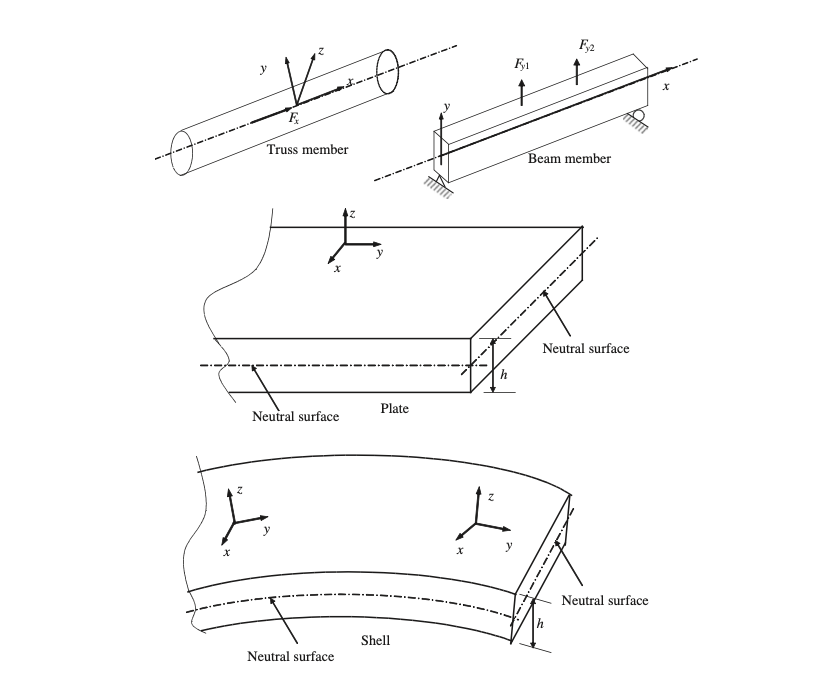
\includegraphics[scale = 0.35]{TypesOfObjects.png}
\end{frame}
\begin{frame}{What to Solve}
    Taking a queue from Liu and Quek, we start off by defining DEE for an idealized infinitesimal, linearly elastic, isotropic material.
    \quad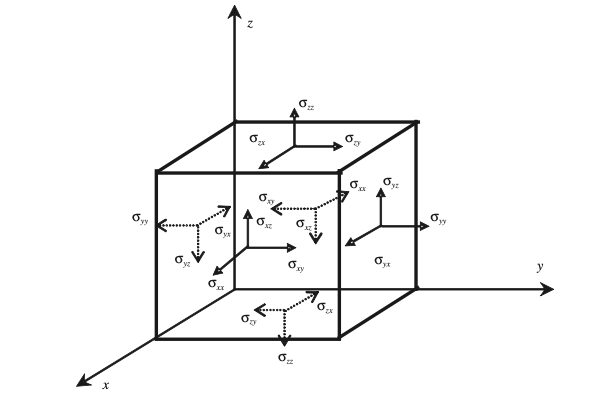
\includegraphics[scale = 0.4]{Cube.png}

    Observe that because of equilibrium $\sigma_{xy} = \sigma_{yx}; \sigma_{xz} = \sigma_{zx}; \sigma_{yz}= \sigma_{yz}$ 
    Which give sus the stress tensors: $\sigma^T = \{\sigma_{xx},\sigma_{yy},\sigma_{zz},\sigma_{yz},\sigma{xz},\sigma{xy}\}$
\end{frame}
\begin{frame}{What to Solve}
    We also get six strain components $\epsilon^T = \{\epsilon_{xx},\epsilon_{yy},\epsilon{zz},\gamma_{yz},\gamma_{xz},\gamma_{xy}$
    Where:
    \begin{align*}
        \epsilon_{xx} &= \frac{\partial u }{\partial x}; \quad \epsilon_{yy} = \frac{\partial v}{\partial y}; \quad \epsilon_{zz} = \frac{\partial w}{\partial z};\\
        \gamma_{xy} &= 2\epsilon_{xy} = \frac{\partial u}{\partial_y} + \frac{\partial v}{\partial x}; \\
        \gamma_{xy} &= 2\epsilon_{xz} = \frac{\partial u}{\partial_z} + \frac{\partial w}{\partial x}; \\
        \gamma_{yz} &= 2\epsilon_{yz} = \frac{\partial v}{\partial_z} + \frac{\partial w}{\partial y}; \\
    \end{align*}
\end{frame}
\begin{frame}{What to Solve}
    Provided $\textbf{U} = \begin{pmatrix}
        u\\
        v\\
        w\\
    \end{pmatrix}$ the displacement matrix we get the system $\epsilon = \textbf{LU}$
    Where the differential operator is:
    $\textbf{L} = \begin{pmatrix}
        \frac{\partial}{\partial x} & 0 & 0\\
        0 & \frac{\partial}{ \partial y} & 0\\
        0 & 0 & \frac{\partial}{\partial z}\\
        0 & \frac{\partial}{\partial z} & \frac{\partial}{\partial y} \\
        \frac{\partial}{\partial z} & 0 & \frac{\partial}{\partial x} \\
        \frac{\partial}{\partial y} & \frac{\partial}{\partial x} & 0 \\
    \end{pmatrix}$

\end{frame}
\begin{frame}{What to solve}
    For an external force in the $y$ direction the equilibrium forces are:
    \begin{dmath}
        (\sigma_{xx}+d\sigma_{xx})dydz - \sigma_{xx}dydz + (\sigma_{yx}+d\sigma_{yx}) dxdz - \sigma_{yx}dxdz + (\sigma_{zx}+d\sigma_{zx})dxdy - \sigma_{zx}dxdy + f_x dx dy dz = \rho \ddot{u} dx dy dz
    \end{dmath}
    But since:
    \begin{align}
        d\sigma_{xx} = \frac{\partial \sigma_{xx}}{\partial x}dx , d\sigma_{yx} = \frac{\partial \sigma_{yx}}{\partial y}dy, d\sigma_{zx} = \frac{\partial \sigma_{zx}}{\partial z} dz
    \end{align}
    Substituting (2) into (1) gives us:
    \begin{align}
        \frac{\partial \sigma_{xx}}{\partial x} + \frac{\partial \sigma_{yx}}{\partial y} + \frac{\partial \sigma_{zx}}{\partial z} + f_x = \rho \ddot{u}
    \end{align}

\end{frame}
\begin{frame}{What to solve}
    Using analogous equations for different directions,$y$ and $z$, we get:
    \begin{align*}
        \frac{\partial \sigma_{xy}}{\partial x} + \frac{\partial \sigma_{yy}}{\partial y} + \frac{\partial \sigma_{zy}}{\partial z} + f_y &= \rho \ddot{v} \\
        \frac{\partial \sigma_{xz}}{\partial x} + \frac{\partial \sigma_{yz}}{\partial y} + \frac{\partial \sigma_{zz}}{\partial z} + f_z &= \rho \ddot{w}
    \end{align*}
    Yielding the linear system:
    \begin{align}
        L^T\sigma + f_b = \rho \ddot{U}
    \end{align}
    And since Hooke's Law states $\sigma = c \epsilon$ we can further simplify to:
    \begin{align*}
        L^TcLU + f_b = \rho \ddot{U}
    \end{align*}
\end{frame}
\begin{frame}{What to Solve}
    For beams, the ruling paradibm is \textit{Euler-Bernoulli} beam theory. This assumes that transverse sections of the beam remain normal to the centroidal axis.
    \begin{center}
    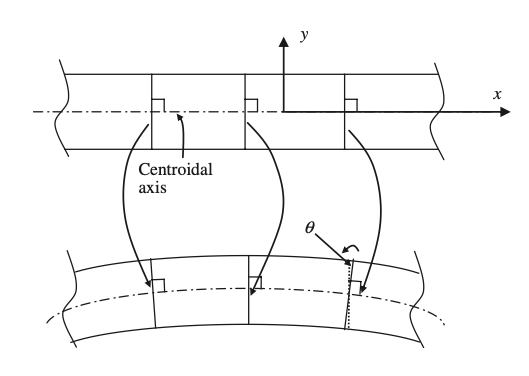
\includegraphics[scale = 0.3]{EBbeam.png}
    \end{center}
    Leads to assumption: $\gamma_{xy} = 0, u = -y\theta, \theta = \frac{\partial v} {\partial x}$
\end{frame}
\begin{frame}{What to Solve}
    Leading us to conclude
    \begin{align}
        \epsilon_{xx} = \frac{\partial u}{\partial x} = \frac{\partial(-y\theta)}{\partial x} = -y\frac{\partial \theta}{\partial x} = -y \frac{\partial^2 v}{\partial x^2} = -yLv
    \end{align}
    With differential operator: $L = \frac{\partial^2}{\partial x^2}$

    Recall that Hooke's Law then says $\sigma_{xx} = E \epsilon_{xx}$
    
    Substituting (5) into Hooke's Law then gives:
    \begin{align}
        \sigma_{xx} = -yELv
    \end{align}
    \newline
    Following further moment derivations from Liu and Quek, the dynamic equilibrium equations for beam is then:
    \begin{align}
        EI \frac{\partial^4 v}{\partial x^4} = F_y
    \end{align}
\end{frame}
\begin{frame}{How to Solve It}
    General structure of a deal.ii step. 
    \begin{enumerate}
        \item include deal.ii headers
        \item Create \texttt{class StepN} with public methods \texttt{StepN(), run()} and private methods \texttt{make_grid(),setup_system(),assemble_system(),solve(),\\output_results()}, and attributes often \texttt{Triangulation<dim>, FE_Q <dim>, DoFHandler<dim>}
        \item Define the methods outside, sometimes all encaspulated in a template for dimension independent programming. 
    \end{enumerate}
\end{frame}
\begin{frame}{How to Solve It}
    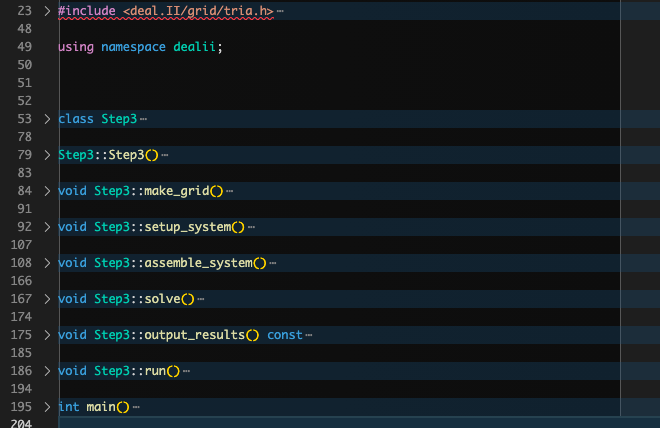
\includegraphics[scale = 0.3]{vscode.png}
\end{frame}
\begin{frame}{How to Solve It}
    Results of solving Laplace Equation on Different Domains:
    \begin{figure}
        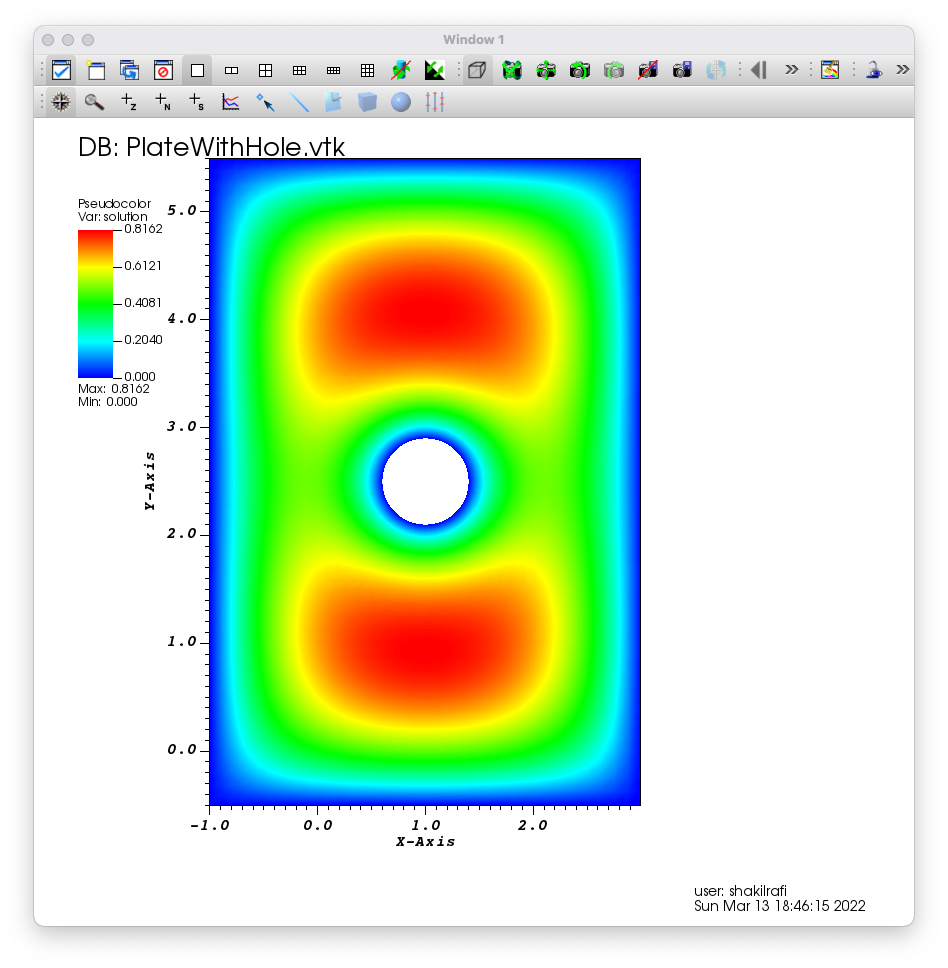
\includegraphics[scale = 0.2]{PlateWithHole.png}
        \caption{Plate with one hole}
    \end{figure} \quad
\end{frame}
\begin{frame}{How to Solve It}
    \begin{figure}
        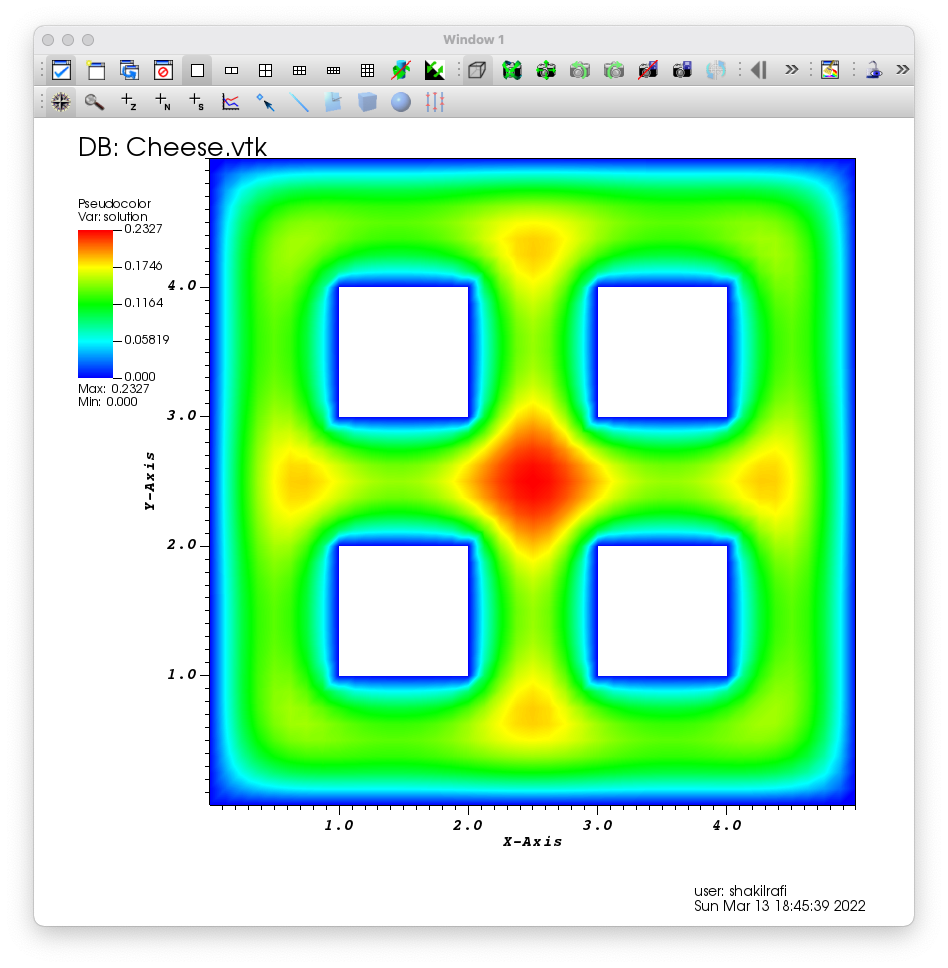
\includegraphics[scale = 0.2]{Cheese.png}
        \caption{Cheese domain}
    \end{figure}
\end{frame}
\begin{frame}{How to Solve It}
    More exotic domains are shown below:

    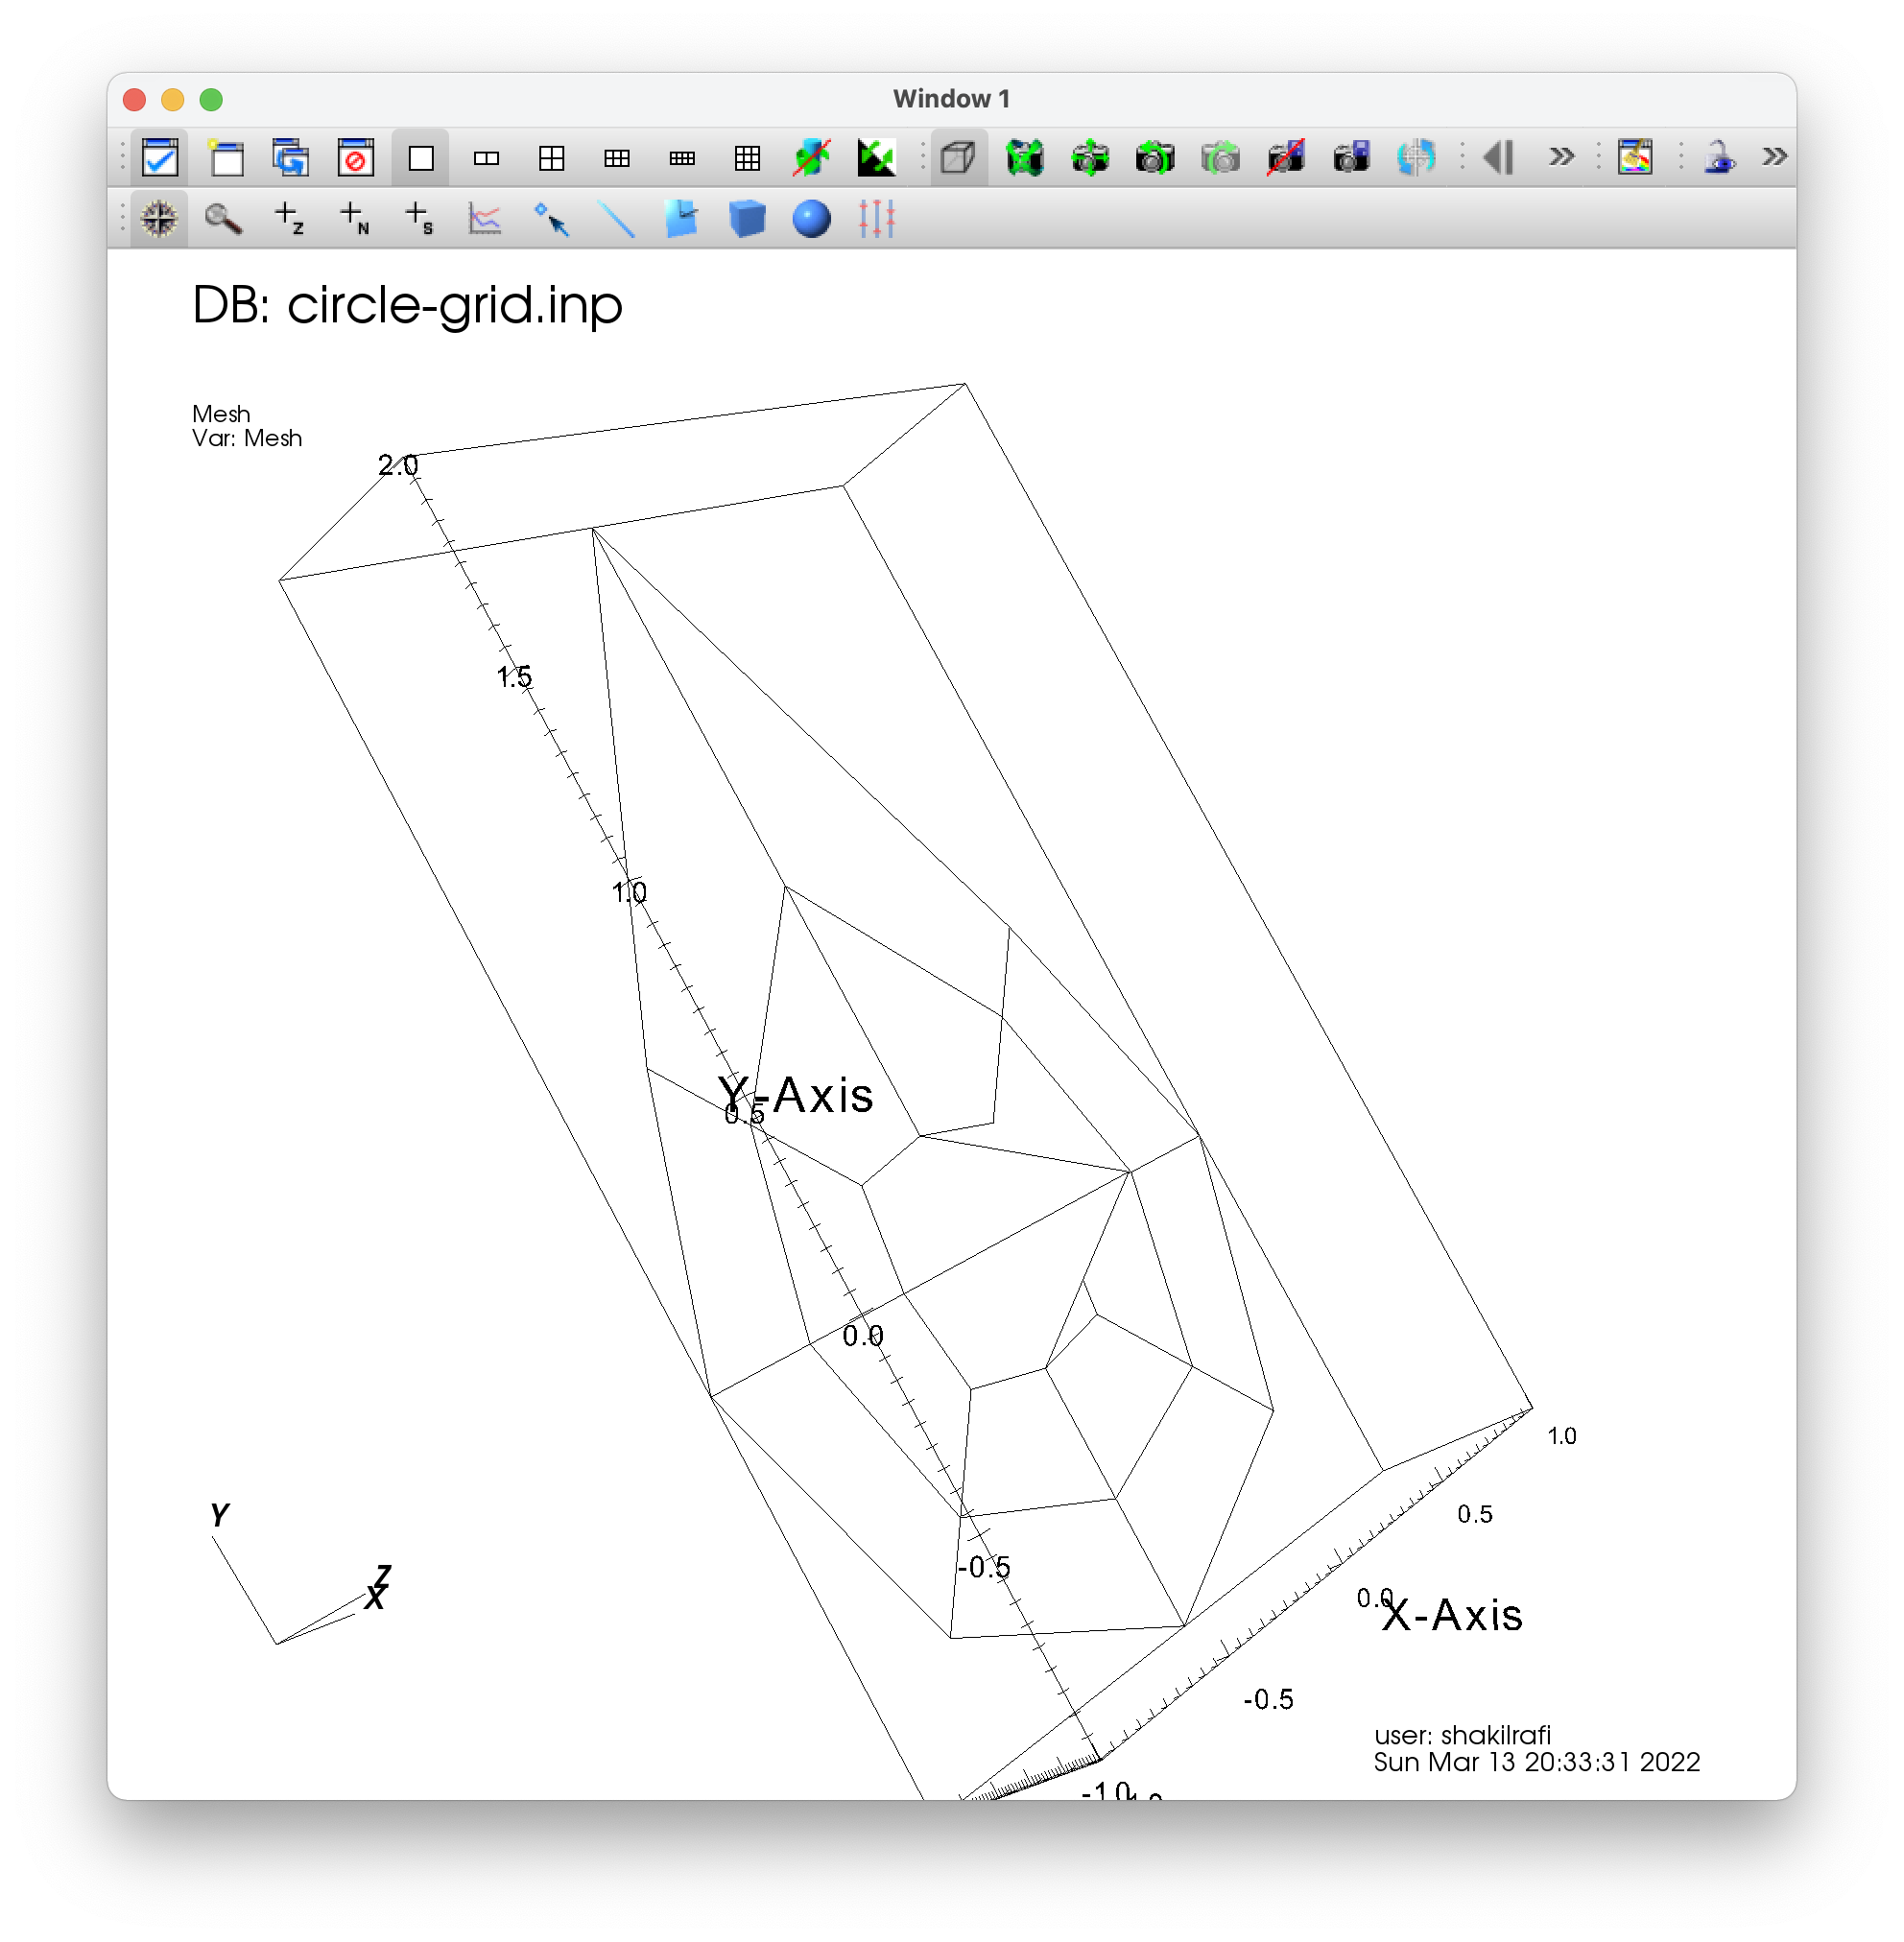
\includegraphics[scale = 0.16]{MFDomain.png}
    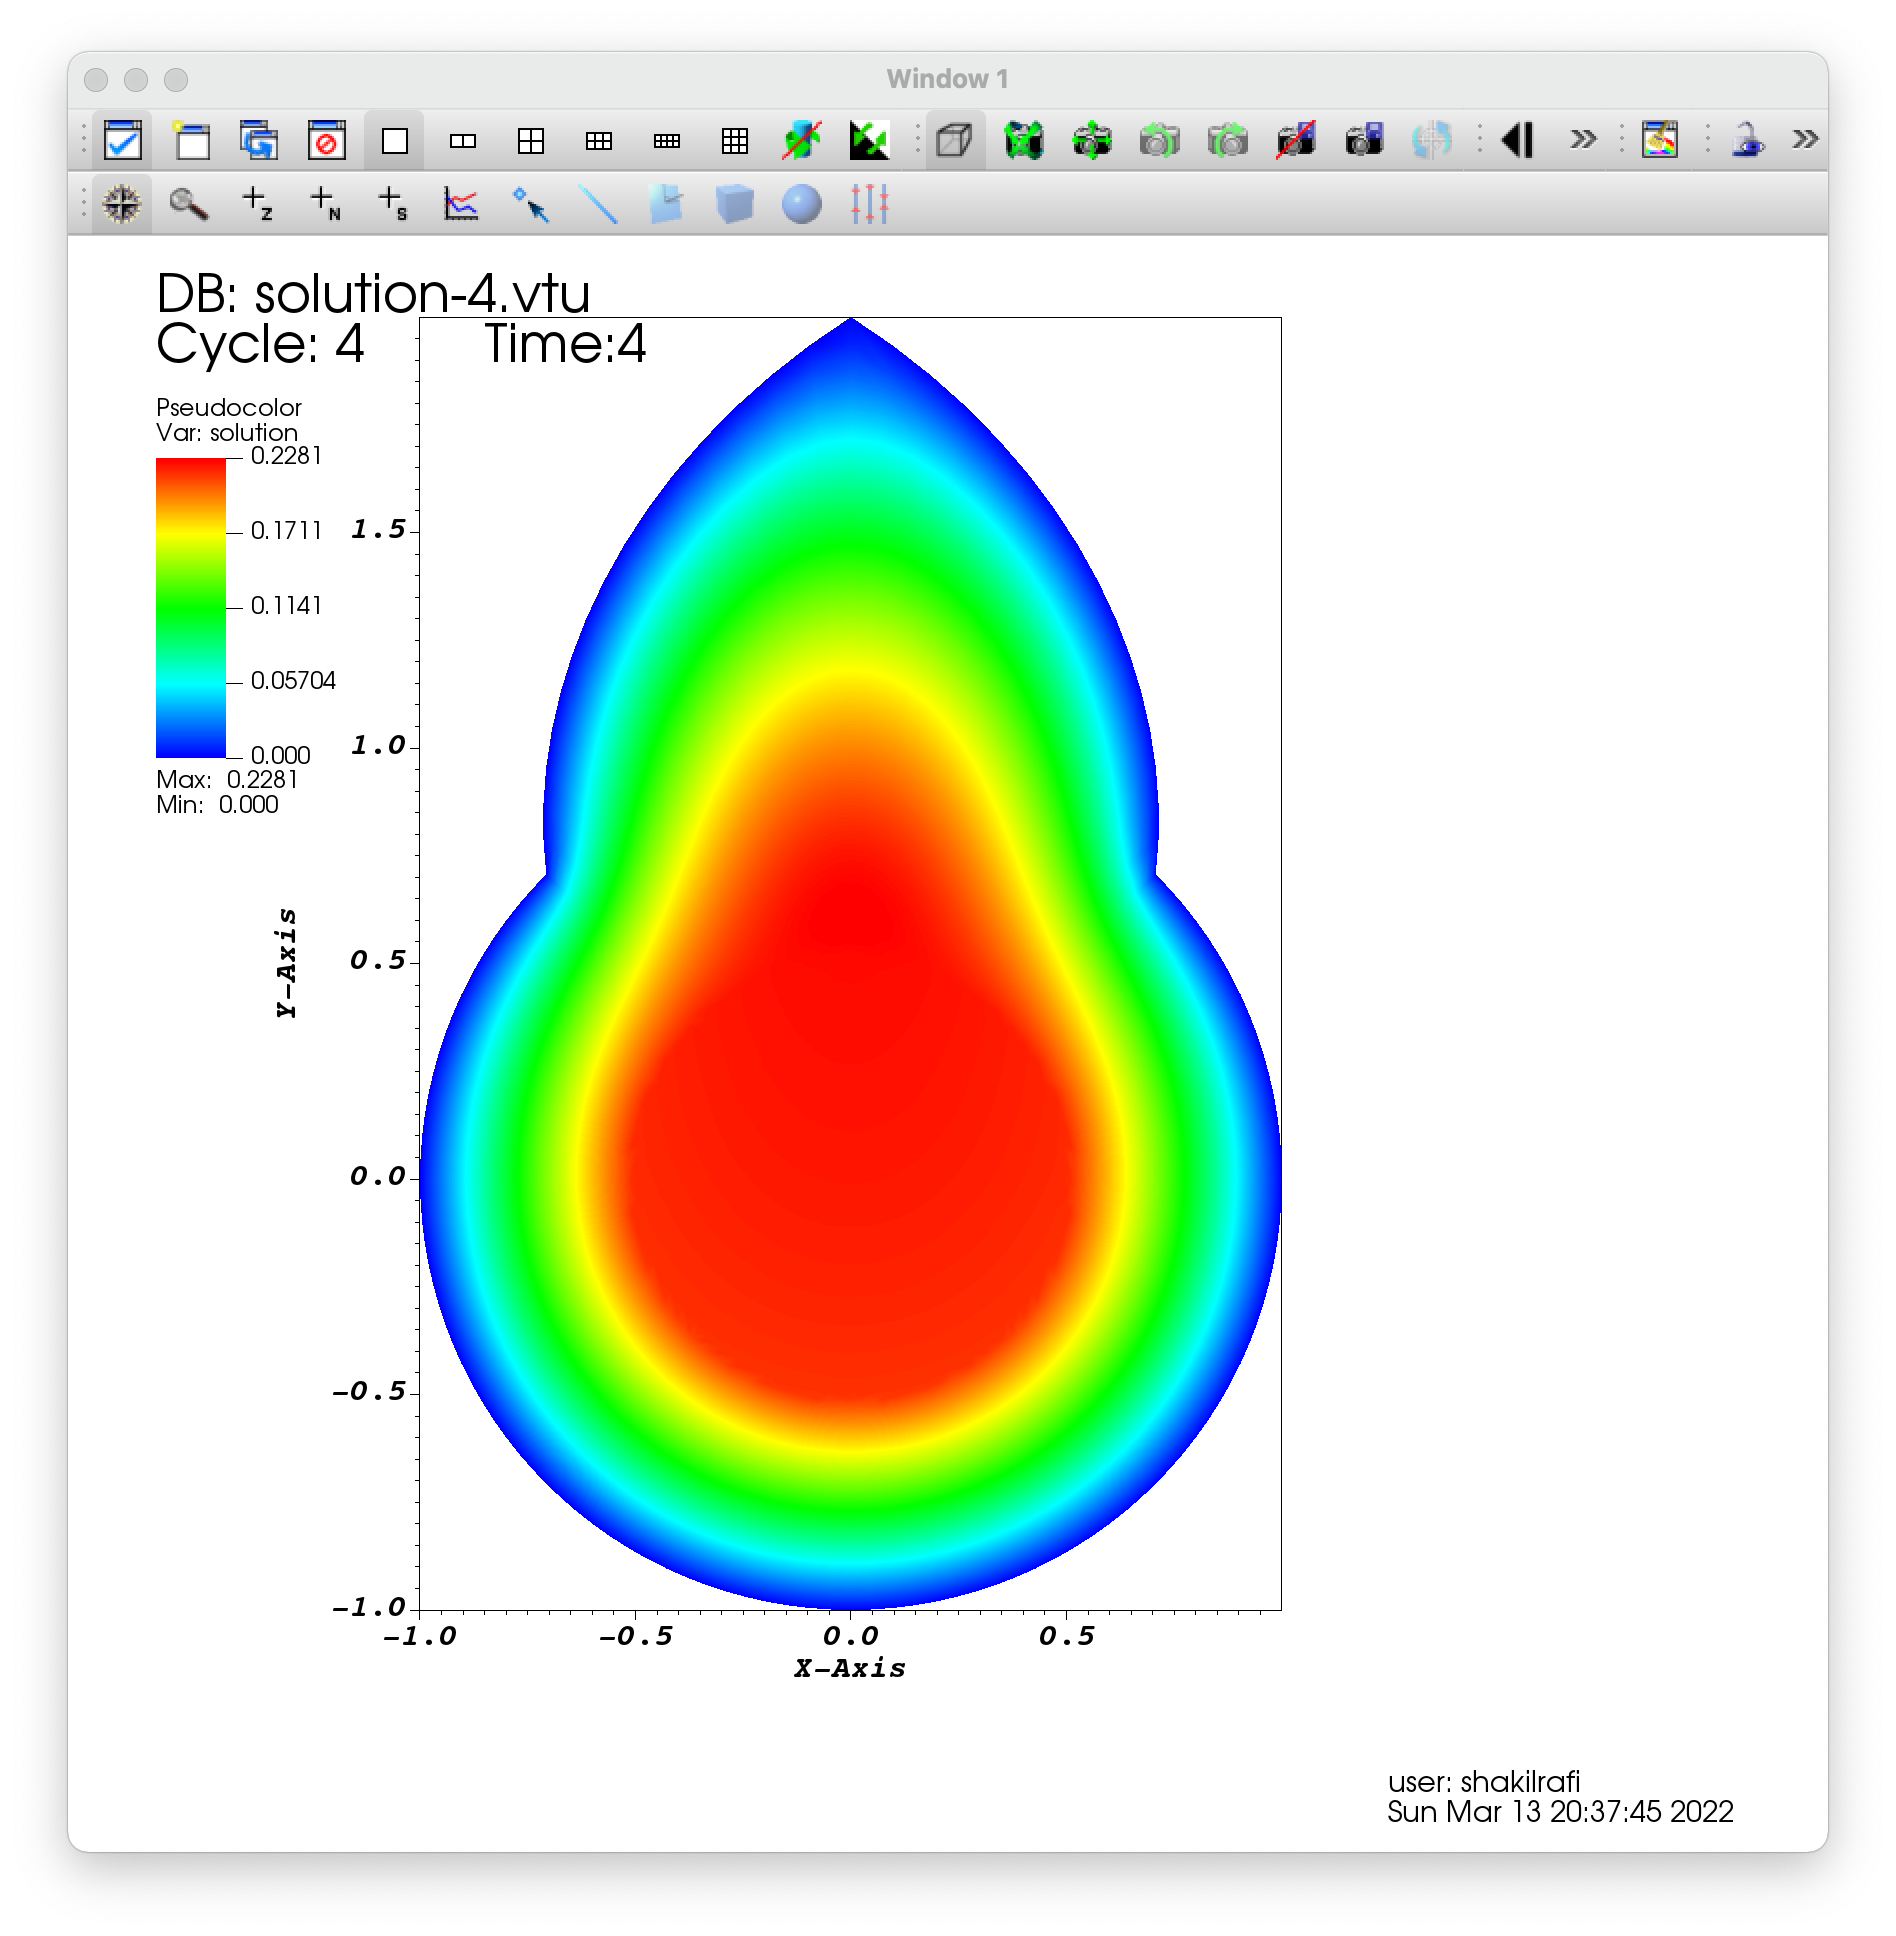
\includegraphics[scale = 0.16]{MFDomainLE.png}
\end{frame}
\begin{frame}{Future Timeline}
    Step-8 deals explicitly with solving linear systems of differential equations. Our next step is to master Step-8. 
    \newline
    \newline
    Step-44 deals exclusively with a certain variation of the dynamic structure equations for a plate. 
    \newline
    \newline
    Mesh data for airplanes from UIUC Airfoil data is not in the format that deal.ii can understand. In particular converting from the Lednicer format in a text file proves challenging and prohibitively time consuming. 
\end{frame}
\end{document}


